% This is samplepaper.tex, a sample chapter demonstrating the
% LLNCS macro package for Springer Computer Science proceedings;
% Version 2.20 of 2017/10/04
%
\documentclass[runningheads]{llncs}
%
\usepackage{graphicx}
\usepackage{csquotes}
\usepackage{hyperref}
\usepackage{fancyvrb}
\usepackage{float}
\usepackage{minted}
\usepackage{cleveref}
% Used for displaying a sample figure. If possible, figure files should
% be included in EPS format.
%
% If you use the hyperref package, please uncomment the following line
% to display URLs in blue roman font according to Springer's eBook style:
% \renewcommand\UrlFont{\color{blue}\rmfamily}

\begin{document}
%
\title{Compiling Haskell: GHC and the Spineless Tagless G-Machine}
%
%\titlerunning{Spineless Tagless G-Machine}
% If the paper title is too long for the running head, you can set
% an abbreviated paper title here
%
\author{Armin Bernstetter}
\date{\today}
%
\authorrunning{Armin Bernstetter}
% First names are abbreviated in the running head.
% If there are more than two authors, 'et al.' is used.
%
\institute{Seminar Funktionale Programmierung \\ Julius-Maximilians-Universität, Würzburg}
%\institute{Princeton University, Princeton NJ 08544, USA \and
%Springer Heidelberg, Tiergartenstr. 17, 69121 Heidelberg, Germany
%\email{lncs@springer.com}\\
%\url{http://www.springer.com/gp/computer-science/lncs} \and
%ABC Institute, Rupert-Karls-University Heidelberg, Heidelberg, Germany\\
%\email{\{abc,lncs\}@uni-heidelberg.de}}
%
\maketitle              % typeset the header of the contribution
%
\begin{abstract}
The Spineless Tagless G-machine (STGM) is an abstract machine that is located at the core of the Glasgow Haskell Compiler GHC. Since its creation at the start of Haskell development in early 1990s it has undergone several significant changes. This work aims at showing the evolution of the STGM and overall at providing insight in the workings of the most widely-used Haskell compiler GHC.

%\keywords{First keyword  \and Second keyword \and Another keyword.}
\end{abstract}
%
%
%

\section{Introduction}

This work provides an insight in the compilation process of the lazy, purely functional programming language Haskell. For this we take a look inside the Glasgow Haskell Compiler, today the most widely-used compiler for Haskell. Located at its core is the \textit{Spineless Tagless G-Machine}, an abstract machine used as a bridge between high level code and machine code.

Described in detail in the 1992 paper \textit{Implementing Lazy functional languages on stock hardware: the Spineless Tagless G-machine} \cite{jones1992implementing}, the STGM has undergone several significant changes since then. Two papers highlighting these changes are \textit{Making a Fast Curry: Push/Enter vs.
Eval/Apply for Higher-order Languages}\cite{marlow2004making} and \textit{Faster Laziness Using Dynamic Pointer Tagging}\cite{marlow2007faster}. The former introducing the switch from the \textit{push-enter} evaluation method to the \textit{eval-apply} model (see \cref{sec:ea}), the latter introducing dynamic pointer tagging which revokes the \enquote{tagless} part in the name of the STGM (see \cref{sec:tagless}).

Section \ref{sec:basics} provides basic information about Haskell, compilers and abstract machines in general.

Section \ref{sec:ghc} describes GHC, the \textit{Glasgow Haskell Compiler} which is the most widely-used Haskell compiler. This section introduces the building blocks that GHC consists of.

Section \ref{sec:stgm} takes a more in-depth look into the \textit{Spineless Tagless G-Machine}, an abstract machine that stands between Haskell code and assembly code in GHC's compilation process. The section shows the state of the STGM in 1992 as well as some changes that have been made since then.

Section \ref{sec:conclusion} concludes with a retrospective overview of STGM and its changes throughout the last 30 years.

\newpage
\section{Basics}
\label{sec:basics}
This section gives some information about the origin of the lazy functional language Haskell. It also introduces some basics about programming language compilers in general and the concept of abstract machines.

\subsection{Haskell}
Haskell is a purely functional programming language that emerged during the late 1980s and early 1990s. It was created with the goal of finding a common functional language to improve interactivity and exchange between programmers and researchers since, at the time, many lesser known functional programming languages existed. A committee consisting of Paul Hudak, John Hughes, Simon Peyton Jones, Philip Wadler and others was created and met several times until in 1990 the Haskell 1.0 Report was published \cite{hudak2007history}. One of the foundations Haskell is based on is the principle of lazy evaluation. Lazy (or non-strict, or call-by-need) evaluation causes compiler development for lazy langauges to differ significantly from strict languages such as C.

\subsection{Compilers}
A compiler is a software system consisting of several phases, that translates programs from a higher-level language to machine code \cite{muchnick1997advanced}.

In general, these phases are \textit{lexical analysis}, \textit{syntactic analysis or parsing}, \textit{semantic checking} and \textit{code generation} \cite{muchnick1997advanced}. Figure \ref{fig:compiler} shows an illustration of these phases and their transitions.

\begin{figure}[h]
\centering
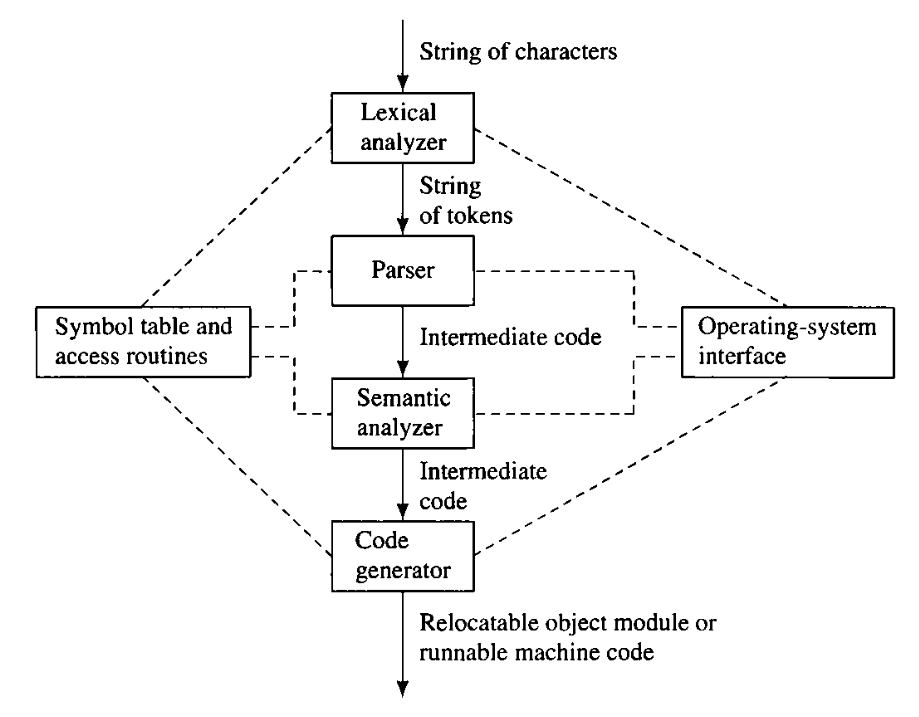
\includegraphics[width=10cm]{compiler.png}
\caption{General illustration of the phases of a compiler taken from Muchnik \cite{muchnick1997advanced}.}
\label{fig:compiler}
\end{figure}

\paragraph{Lexical Analysis} analyzes the character string and produces errors in case any part of the program string is not parseable into legal tokens. Legal in this case refers to tokens that are members of the vocabulary of the respective programming language.

\paragraph{Syntactic Analysis/Parsing} parses the program into an intermediate representation. An example would be a parse tree accompanied by a symbol table containing information on identifiers used in the program and their attributes. This phase may also produce error messages if syntax errors are detected.

\paragraph{Semantic Checking} examines the program for static-semantic validity. This phase takes as input the intermediate representation and determines whether the program satisfies the requirements for the static-semantic properties of the source language.

\paragraph{Code Generation} finally transforms the intermediate representation into machine code which can then be executed. 


These phases are often complemented by additional steps in many compilers, the Glasgow Haskell Compiler being one of those (see Section \ref{sec:ghc}).

\subsection{Abstract Machines}
Abstract machines bridge the gap between high level source code and machine code by providing an intermediate language stage for compilation. They are located in the conceptual space between the two extremes of being a small intermediate language and being a model for a real machine that is yet to be built \cite{diehl2000abstract}.

Abstract machines execute programs step-by-step in a loop. This execution loop iterates over a sequence of instructions often using a stack and register with the program counter as a special register pointing at the next instruction. \cite{diehl2000abstract}

These machines introduce an additional layer of abstraction to the implementation of compilers for programming languages.

Examples for such abstract machines or related concepts are the Java Virtual Machine and the Spineless Tagless G-Machine which is the focus of this work.

\section{GHC}
\label{sec:ghc}
The Glasgow Haskell Compiler, named after the city where its development began in 1989, is the most widely-used Haskell compiler \cite{marlow2007faster}. It is the de facto default compiler for Haskell and is shipped with the \textit{Haskell Platform} downloadable at \url{https://www.haskell.org/}.

Figure \ref{fig:ghc} illustrates the different phases program code is passed through during compilation. In contrast to the general compiler structure shown in figure \ref{fig:compiler}, GHC has several additional intermediate steps. 

The Haskell source code is initially parsed and translated to a reduced \textit{Core} language which is then again translated to the \textit{STG representation}. A code generator (the \textit{STGM}) generates \texttt{C--} code followed by three possible paths for finally generating machine code.

\begin{figure}

\centering
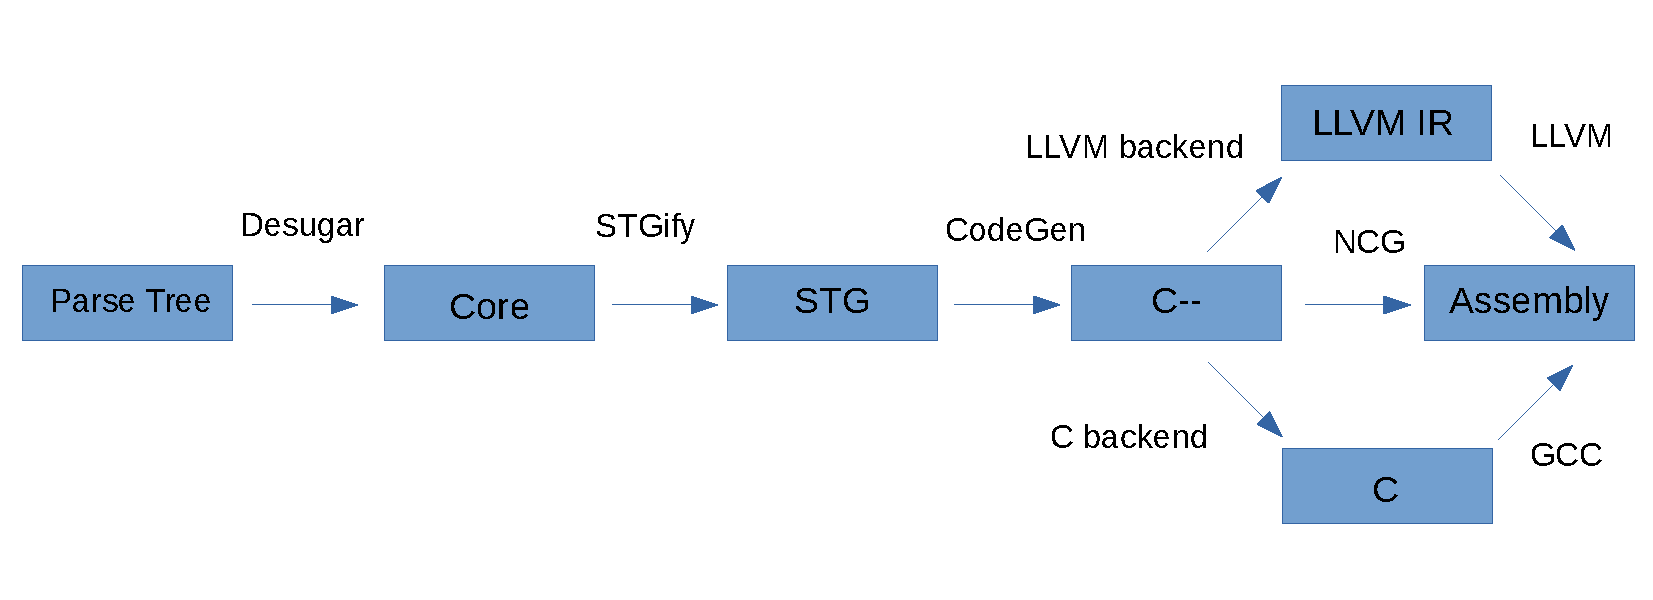
\includegraphics[width=12cm]{ghcflow.pdf}
\caption{GHC's compilation phases. Own graphic based on a depiction from the official GHC repository \protect\footnotemark}
\label{fig:ghc}
\end{figure}
\footnotetext{\url{https://gitlab.haskell.org/ghc/ghc/wikis/commentary/compiler/generated-code}}

\subsection{Core Language}
The core language is a variant of Haskell in where all syntactic sugar is removed and resolved e.g. the do-notation or type aliases. It consists of Haskell's central data types and is a small, explicitly-typed variant of the typed lambda calculus System F \cite{girard1986system} which is called System FC \cite{sulzmann2007system}. Type checking is performed here, overloading is resolved and pattern-matching is translated into \texttt{case} expressions where each one performs only a single level of matching \cite{jones1992implementing}.

\subsection{The STG Language}
The core language is then translated to the \textit{STG language}.
This language is a purely functional programming language on its own that is used as an intermediate representation.

Some of its characteristics defined by Peyton Jones \cite{jones1992implementing} are:

\begin{itemize}
	\item[] \textit{All function and constructor arguments are simple variables or constants.}
	\item[] \textit{All constructors and built-in operations are saturated.}
	\item[] \textit{Pattern matching is performed only by \texttt{case} expressions.}
\end{itemize}

Each of the constructs in the language corresponds to an operational reading.
Each \texttt{let} expression allocates an object in the heap. The nature of heap objects is expanded on in section \ref{sec:stgm}. A \texttt{case} expression forces evaluation of a sub-expression. A function application represents a tail call and a constructor application represents the return to a continuation. 

\begin{table}[H]
	\centering
	
	\begin{tabular}{|l|l|}
		\hline 
		Construct & Operational reading  \\ 
		\hline 
		Function application	& Tail call  \\  
		\texttt{let} expression	& Heap allocation  \\ 
		\texttt{case} expression	& Evaluation  \\ 
		Constructor application	& Return to continuation  \\ 
		\hline 
	\end{tabular} 
	\caption{Table taken from Jones 1993 \cite{jones1992implementing}}
\end{table}

Section \ref{sec:stgm} will go into further detail on the syntax of the intermediate STG language.

\subsection{\texttt{C--}}
\label{subsec:C--}

A code generator (the STG machine) translates the STG language into \texttt{C--}. In fact, in Peyton Jones's 1992 paper \cite{jones1992implementing} this step generated an intermediate representation called \textit{Abstract C}. It was only several years later that \texttt{C--} came into being \cite{jones1999c}.

\texttt{C--} is a programming language developed by Simon Peyton-Jones as a portable backend-language for compilers. Where C++ can be seen as an extension of the C language, \texttt{C--} is to be thought of as a reduction to a smaller core language. \texttt{C--} in general is made for being generated by compilers and not for being written by programmers. \cite{jones1999c}

\subsection{Backends}
GHC supports the generation of assembly machine code via multiple backends. In addition to a native code generator it offers a compilation route via LLVM and a route via C that has, however, been deprecated.

\subsubsection{Native Code Generator}
The Native Code Generator is the default backend used in GHC and compiles \texttt{C--} directly to assembly code. The NCG is the fastest backend and produces well performing code. \cite{GHCmanual}

\subsubsection{LLVM}
LLVM is a modern portable compiler framework that was developed as an alternative to the classic GCC toolchain. Its acronym stands for \textit{Low Level Virtual Machine} \cite{lattner2004llvm}.

Using LLVM in GHC results in similar compilation performance as the NCG but can lead to faster performing executables for some cases. In these cases - like numeric, array heavy code - the penalty is a significant increase in compilation times, though. To use GHC with the LLVM backend, LLVM has to be installed on the respective system.\cite{GHCmanual}

\subsubsection{C Backend}
The C backend uses the \textit{GNU Compiler Collection} GCC but has bee deprecated since around GHC version 7.0 (2011) \cite{GHCmanual}.





\section{The STGM in depth}
\label{sec:stgm}

The Spineless Tagless G-Machine is an abstract machine for non-strict functional languages.
It was developed by Simon Peyton Jones as an alternative or successor to other such abstract machines like the \textit{Three Instruction Machine (TIM)} by Fairbairn and Wray \cite{fairbairn1987tim} and the \textit{G-Machine} by Johnsson \cite{johnsson1984efficient}.
The STG machine transforms the incoming code from the core language to \texttt{C--} via the intermediate STG language.






\subsubsection{Closures}
Heap objects can be either evaluated \textit{head normal forms} (\textit{values}) or unevaluated suspensions (\textit{thunks}).

In the context of the STGM, the term \textit{closure} refers to both values and thunks.

Such closures are represented as a pointer to a contiguous block of heap-allocated storage which consists of a \textit{pointer} pointing to the static code, followed by the values of any free variables.


\subsubsection{Heap Objects}

There are five kinds of heap objects in the STG language \cite{marlow2004making}.

\begin{itemize}
	\item[] $FUN(x_1 \dots x_n \rightarrow e)$: A function closure \textit{FUN} has $n$ arguments and a body $e$. Such a function may be applied to more or fewer than $n$ arguments but still has an \textit{arity} of n i.e. it is \textit{curried}.
	\item[] $PAP(f a_1 \dots a_n)$: A partial application \textit{PAP} represents a function \textit{f} that is applied to \textit{n} arguments $x_i$. The function $f$ is a \textit{FUN} object and its \textit{arity} is strictly greater than \textit{n}.
	\item[] $CON(C a_1 \dots a_n)$: A constructor object \textit{CON} represents a data value. The constructor \textit{C} is applied to $n$ arguments. This application is always saturated, that means the arity of \textit{C} is always equal to the number of arguments.
	\item[] $THUNK e$: A Thunk is an unevaluated expression, also called \textit{suspension}. A thunk is evaluated and overwritten with the value of \textit{e} when this value is needed.
	\item[] $BLACKHOLE$: Is an object that is only used during the evaluation of a thunk. It replaces the thunk to prevent e.g. space leaks.
\end{itemize}

Listings \ref{lst:map1} and \ref{lst:map2} show an implementation of a \texttt{map} function in Haskell and its representation in the STG language respectively.

\begin{listing}[H]
\begin{minted}[baselinestretch=0.5]{Haskell}
map f []     = []

map f (x:xs) = f x : map f xs
\end{minted}
\caption{A \texttt{map} function implemented in Haskell.}
\label{lst:map1}
\end{listing}

\begin{listing}[H]
\begin{minted}[baselinestretch=0.5]{Haskell}
nil = CON Nil

map = FUN (f xs ->

        case xs of

           Nil -> nil

           Cons y ys -> let h = THUNK (f y)

                            t = THUNK (map f ys)

                            r = CON (Cons h t)

                        in r

     )
\end{minted}
\caption{The map function from listing \ref{lst:map1} represented in the STG language}
\label{lst:map2}
\end{listing}

\subsubsection{\enquote{Spineless}}
The term \enquote{spineless} refers to the way the STG code is represented on the machine. 

STG programs are not represented as a tree but as a graph. Therefore, in memory a STG program is not a contiguous block of memory but smaller parts of the graph that reference each other and can be shared (common subexpressions).

The STGM is based on \textit{graph reduction}, a concept first introduced in a Ph.D. dissertation by Christopher Wadsworth in 1971 \cite{christopherwadsworth}. Henderson et al. continued this concept in 1976 by presenting a different and lazy way to execute LISP programs \cite{henderson1976lazy} which was then again the basis for lazy functional programming languages including Haskell. Wadsworth suggested a graph-reduction strategy that used pointers to implement sharing of closures.

\subsubsection{\enquote{Tagless}}
\label{sec:tagless}
The term tagless refers to the way the STG-machine evaluates a heap closure.
All heap objects have a uniform representation with a code pointer in their first field. This is true for both unevaluated suspensions and head normal forms. The STGM does not examine tag fields in those objects to decide how to treat them but rather makes a jump to the code pointed to. \cite{jones1992implementing}

This concept is explained in an example by Marlow et al. \cite{marlow2007faster}. Take for example the expression

\begin{center}
	\begin{BVerbatim}
	f x y = case x of (a,b) -> a + y
	\end{BVerbatim}
\end{center}

The compiler of a lazy language has to ensure that \texttt{x} is evaluated before taking it apart into patterns. It pushes a continuation for the computation \texttt{a+y} onto the stack and jumps to the \textit{entry code} for \texttt{x}. This jump to the entry code is called \textit{entering} the closure. If the closure is unevaluated, the entry code will evaluate it and return its value to the continuation, otherwise it will return immediately.
A tag-ful approach would only enter the closure if it is not yet evaluated. This would be checked by performing an extra test on the tag i.e. the type of the closure. The benefit of a tagless approach is that any closure can be evaluated simply by entering it which is a simple and uniform process. \cite{marlow2007faster}



\subsection{Function Application}
Function calls in a lazy functional languages with currying and partial application require special mechanisms in compilers. Showing how function application is performed provides much insight into the compilation strategy of a language like Haskell.

\textit{Currying} is one of the core principles of lazy functional languages such as Haskell. A function
\begin{center}
\begin{BVerbatim}
f x y = x
\end{BVerbatim}
\end{center}
has the type \texttt{a -> (b -> a)}. It can be seen as a function which takes one argument and returns a function which takes the second argument. An application like \texttt{(f 1 2)} is short for \texttt{((f 1) 2)}. Applying \texttt{f} to only one argument is a valid expression and is called \textit{partial application}.

Compilers based on lazy graph reduction often compile function application using a strategy called the \textit{push-enter model}. This model was used by the STG machine initially. The basic principle is that the argument(s) given to a function are \textit{pushed} on an evaluation stack and then the function is tail-called (or \textit{entered})\cite{jones1992implementing}.



Consider the program shown in listing \ref{lst:apply}. This short program is taken from the code examples of the \textit{Ministg} project. This project \enquote{is an interpreter for a high-level, small-step, operational semantics for the STG machine} by developer Bernie Pope. Its repository can be found on \url{https://github.com/bjpop/ministg}.

It offers functionality for tracing the evaluation steps which the STG machine takes to evaluate function application.

\begin{listing}[H]
	\begin{minted}[baselinestretch=0.5]{Haskell}
	const = FUN(x y -> x);
	
	apply = FUN(f x -> f x);b
	
	true = CON(True);
	twentytwo = CON(I 22);
	
	main = THUNK(apply const true twentytwo)
	
	\end{minted}
	\caption{An example program \texttt{apply.stg} written in STG syntax.}
	\label{lst:apply}
\end{listing}

The program shown in listing \ref{lst:apply} simply returns \texttt{true}. The function \texttt{const} takes two arguments, throws away the second and returns the first. The function \texttt{apply} takes a function \texttt{f} and another argument \texttt{x} and returns the function \texttt{f} applied to \texttt{x}. \texttt{twentytwo} is a constructor value that represents the integer \textit{22} and \texttt{true} is a constructor that represents the boolean value \texttt{True}. The program \texttt{main} is a \texttt{THUNK} i.e. an expression, which is yet to be evaluated.



\Cref{tb:pe_step0,tb:pe_step1,tb:pe_step2,tb:pe_step3,tb:pe_step4,tb:pe_step5,tb:pe_step6} show the evaluation trace for the program shown in \cref{lst:apply} when using the \textit{push-enter-model} of evaluation.
The tables on the left show the arguments that are currently on the stack as well as the next expression to be evaluated. The tables on the right show the objects which are currently allocated on the heap and their variable names. Each table's caption names the most recent evaluation rule that has been applied in bold script. For more details on the meaning of those rules see \textit{Making a Fast Curry: Push/Enter vs. Eval/Apply for Higher-order Languages} by Simon Marlow and Simon Peyton Jones \cite{marlow2004making}.

\begin{table}[H]
\begin{tabular}{lll}
\begin{tabular}{|l|l|}
	\multicolumn{2}{c}{\textbf{Stack and Code}}  \\
	\hline 
	\textbf{Stack} & \textbf{Expression} \\ 
	\hline 
	& \texttt{main} \\ 
	\hline 
\end{tabular} 	
& &
\begin{tabular}{|l|l|}
	\multicolumn{2}{c}{\textbf{Heap}}  \\ 
	\hline 
	\textbf{Variable} & \textbf{Object} \\ 
	\hline 
	\texttt{apply}&  \texttt{FUN(f x -> f\_? x)}\\ 
	\texttt{const}& \texttt{FUN(x y -> x)} \\
	\texttt{main}& \texttt{THUNK(apply\_2 const true twentytwo)}\\
	\texttt{true}&\texttt{CON(True)}\\
	\texttt{twentytwo}&\texttt{CON(I 22)}\\
	\hline
\end{tabular} 
\end{tabular}
\vspace*{5mm}
\caption{The objects have been allocated on the heap and the expression \texttt{main} is next to be evaluated.}
\label{tb:pe_step0}
\end{table}
\vspace{-5em}
\begin{table}[H]
	\begin{tabular}{lll}
		\begin{tabular}{|l|l|}
			\multicolumn{2}{c}{\textbf{Stack and Code}}  \\
			\hline 
			\textbf{Stack} & \textbf{Expression} \\ 
			\hline 
			\texttt{upd * main}& \texttt{apply\_2 const true twentytwo} \\ 
			\hline 
		\end{tabular} 	
		& &
		\begin{tabular}{|l|l|}
			\multicolumn{2}{c}{\textbf{Heap}}  \\ 
			\hline 
			\textbf{Variable} & \textbf{Object} \\ 
			\hline 
			\texttt{apply}&  \texttt{FUN(f x -> f\_? x)}\\ 
			\texttt{const}& \texttt{FUN(x y -> x)} \\
			\texttt{main}& \texttt{BLACKHOLE}\\
			\texttt{true}&\texttt{CON(True)}\\
			\texttt{twentytwo}&\texttt{CON(I 22)}\\
			\hline
		\end{tabular} 
	\end{tabular}
	\vspace*{5mm}
	\caption{\textbf{THUNK (most recent rule applied):} \texttt{main} is a thunk and has therefore been replaced by a \texttt{BLACKHOLE} on the heap during its evaluation. \texttt{upd * main} which is currently on the stack will eventually update \texttt{main} with its value. The next expression to be evaluated is \texttt{apply\_2 ...}, a function of \textit{arity} 2 which is given three arguments.}
	\label{tb:pe_step1}
\end{table}
\newpage
\begin{table}[H]
	\begin{tabular}{lll}
		\begin{tabular}{|l|l|}
			\multicolumn{2}{c}{\textbf{Stack and Code}}  \\
			\hline 
			\textbf{Stack} & \textbf{Expression} \\ 
			\hline 
			\texttt{arg const}& \texttt{apply} \\ 
			\texttt{arg true}& \\
			\texttt{arg twentytwo}& \\
			\texttt{upd * main}& \\
			\hline 
		\end{tabular} 	
		& &
		\begin{tabular}{|l|l|}
			\multicolumn{2}{c}{\textbf{Heap}}  \\ 
			\hline 
			\textbf{Variable} & \textbf{Object} \\ 
			\hline 
			\texttt{apply}&  \texttt{FUN(f x -> f\_? x)}\\ 
			\texttt{const}& \texttt{FUN(x y -> x)} \\
			\texttt{main}& \texttt{BLACKHOLE}\\
			\texttt{true}&\texttt{CON(True)}\\
			\texttt{twentytwo}&\texttt{CON(I 22)}\\
			\hline
		\end{tabular} 
	\end{tabular}
	\vspace*{5mm}
	\caption{\textbf{PUSH:} The arguments \texttt{const}, \texttt{true} and \texttt{twentytwo} have been pushed onto the stack. The next expression to be evaluated is \texttt{apply}.}
	\label{tb:pe_step2}
\end{table}
\begin{table}[H]
	\vspace{-5em}
	\begin{tabular}{lll}
		\begin{tabular}{|l|l|}
			\multicolumn{2}{c}{\textbf{Stack and Code}}  \\
			\hline 
			\textbf{Stack} & \textbf{Expression} \\ 
			\hline 
			\texttt{arg twentytwo}& \texttt{const\_? true} \\ 
			\texttt{upd * main}& \\
			\hline 
		\end{tabular} 	
		& &
		\begin{tabular}{|l|l|}
			\multicolumn{2}{c}{\textbf{Heap}}  \\ 
			\hline 
			\textbf{Variable} & \textbf{Object} \\ 
			\hline 
			\texttt{const}& \texttt{FUN(x y -> x)} \\
			\texttt{main}& \texttt{BLACKHOLE}\\
			\texttt{true}&\texttt{CON(True)}\\
			\texttt{twentytwo}&\texttt{CON(I 22)}\\
			\hline
		\end{tabular} 
	\end{tabular}
	\vspace*{5mm}
	\caption{\textbf{FENTER:} the function \texttt{apply} has been \textit{entered} and returned the expression \texttt{const\_? true}. These are the two arguments that \texttt{apply} \enquote{took} from the stack. \texttt{const\_?} is of yet unknown arity.}
	\label{tb:pe_step3}
\end{table}
\begin{table}[H]
	\vspace{-5em}
	\begin{tabular}{lll}
		\begin{tabular}{|l|l|}
			\multicolumn{2}{c}{\textbf{Stack and Code}}  \\
			\hline 
			\textbf{Stack} & \textbf{Expression} \\ 
			\hline 
			\texttt{arg true}& \texttt{const} \\ 
			\texttt{arg twentytwo} & \\
			\texttt{upd * main}& \\
			\hline 
		\end{tabular} 	
		& &
		\begin{tabular}{|l|l|}
			\multicolumn{2}{c}{\textbf{Heap}}  \\ 
			\hline 
			\textbf{Variable} & \textbf{Object} \\ 
			\hline 
			\texttt{const}& \texttt{FUN(x y -> x)} \\
			\texttt{main}& \texttt{BLACKHOLE}\\
			\texttt{true}&\texttt{CON(True)}\\
			\texttt{twentytwo}&\texttt{CON(I 22)}\\
			\hline
		\end{tabular} 
	\end{tabular}
	\vspace*{5mm}
	\caption{\textbf{PUSH:} The argument \texttt{true} that \texttt{const\_?} was applied to has been pushed onto the stack. The next expression to be evaluated is \texttt{const}.}
	\label{tb:pe_step4}
\end{table}

\begin{table}[H]
	\vspace{-5em}
	\begin{tabular}{lll}
		\begin{tabular}{|l|l|}
			\multicolumn{2}{c}{\textbf{Stack and Code}}  \\
			\hline 
			\textbf{Stack} & \textbf{Expression} \\ 
			\hline 
	
			\texttt{upd * main}& \texttt{true} \\
			\hline 
		\end{tabular} 	
		& &
		\begin{tabular}{|l|l|}
			\multicolumn{2}{c}{\textbf{Heap}}  \\ 
			\hline 
			\textbf{Variable} & \textbf{Object} \\ 
			\hline 
			\texttt{main}& \texttt{BLACKHOLE}\\
			\texttt{true}&\texttt{CON(True)}\\
			\hline
		\end{tabular} 
	\end{tabular}
	\vspace*{5mm}
	\caption{\textbf{FENTER:} \texttt{const} now has found the remaining two arguments it needed on the stack and returned the first of them, \texttt{true}.}
	\label{tb:pe_step5}
\end{table}
\begin{table}[H]
	\vspace{-5em}
	\begin{tabular}{lll}
		\begin{tabular}{|l|l|}
			\multicolumn{2}{c}{\textbf{Stack and Code}}  \\
			\hline 
			\textbf{Stack} & \textbf{Expression} \\ 
			\hline 
						& \texttt{true} \\
			\hline 
		\end{tabular} 	
		& &
		\begin{tabular}{|l|l|}
			\multicolumn{2}{c}{\textbf{Heap}}  \\ 
			\hline 
			\textbf{Variable} & \textbf{Object} \\ 
			\hline 
			\texttt{true}&\texttt{CON(True)}\\
			\hline
		\end{tabular} 
	\end{tabular}
	\vspace*{5mm}
	\caption{\textbf{UPDATE:} the expression \texttt{true} has been evaluated and is the new value that the thunk \texttt{main} has been updated with. The computation is now finished.}
	\label{tb:pe_step6}
\end{table}
\newpage
\subsection{Changes since 1992}
The Glasgow Haskell Compiler and in consequence its several intermediate phases are in constant development. As a result, the Spineless Tagless G-Machine has undergone multiple changes since Simon Peyton Jones's paper in 1992 \cite{jones1992implementing}. 

Two of the more impactful changes were the switch from the aforementioned \textit{push-enter} model for function evaluation to the \textit{eval-apply} model and the discarding of the \enquote{tagless} aspect of the Spineless Tagless G-machine.

\subsubsection{Function application: Eval-Apply}
\label{sec:ea}
In 2004, Marlow and Peyton Jones\cite{marlow2004making} reevaluated the choice for the \textit{push-enter} model for function application . They found, that the \textit{eval-apply} model, which had initially been discarded \cite{jones1992implementing} actually delivered better compilation performance.

\textit{Eval-apply} is a model which originated from compilers from the Lisp tradition. In this model, the basic principle is to first evaluate the function, then evaluate the argument and apply the function value to the argument \cite{jones1992implementing}. The \textit{caller} of a function knows at the time of calling what the arguments are. It examines the function closure, extracts its arity, and makes an exact call to the function \cite{marlow2004making}. This places the responsibility of matching the \textit{arity} of the function to the number of arguments in the call on the \textit{caller}. In the \textit{push-enter} model this responsibility lies with the \textit{function} itself.

\Cref{appA} shows the evaluation trace of the \texttt{apply.stg} program  from \cref{lst:apply} for the \textit{eval-apply} model in tables \cref{tb:ea_step0,tb:ea_step1,tb:ea_step2,tb:ea_step3,tb:ea_step4,tb:ea_step5,tb:ea_step6,tb:ea_step7}.


\subsubsection{Dynamic Pointer Tagging}
In 2007, Marlow et al. \cite{marlow2007faster} found that Haskell programs compiled by GHC show mispredicted branches on modern processors. This led to a re-examination of the \enquote{tagless} aspect of the STGM. The result were significant performance improvements.

The drawback of the taglessness described in \cref{sec:tagless} is that it comes at the expense of performing indirect jumps. One jump is needed to enter the closure and another to return to the evaluation site. Indirect jumps like these are expensive on modern processors, because they confuse the branch-prediction hardware which leads to a stall of several cycles. \cite{marlow2007faster}

If a closure is unevaluated, an indirect jump has to be taken. If the closure is already evaluated, however, conditional jumps execute faster as Marlow et al. showed with several approaches \cite{marlow2007faster}. Two of their strategies were \textit{semi-tagging} and \textit{dynamic pointer tagging}.

\Cref{fig:obj} shows the uniform representation of any heap object. The first word is an \textit{info pointer} pointing to the associated \textit{entry code} and the \textit{info table} of the object. The info table describes the layout the type of the object (constructor, thunk, function, \dots). If an object is a data constructor, another field gives the \textit{tag} of the constructor.

\begin{figure}[H]
\begin{center}
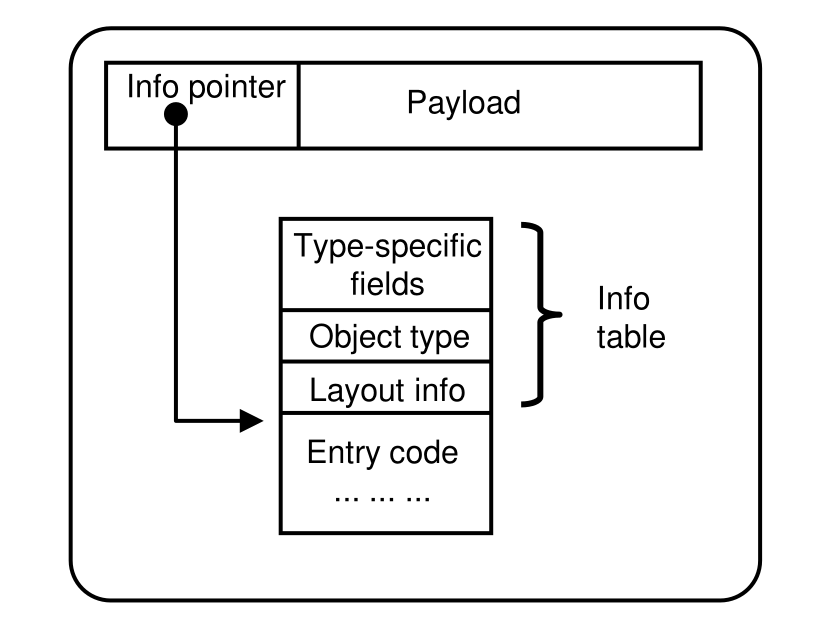
\includegraphics[width=8cm]{heapobject.png}
\end{center}
\caption{A heap object (graphic taken from \cite{marlow2007faster}).}
\label{fig:obj}

\end{figure}


\paragraph{Semi-tagging} is a scheme that produces code that does not enter already evaluated code. It tests the type of the closure before entering by looking at the info table. If it is a constructor it continues directly with the code to examine the constructor. If it is unevaluated the closure is entered and evaluated.

\paragraph{Pointer-tagging} encodes the information about evaluatedness and the tag of a closure directly in the \textit{info pointer} to the closure. This avoids dereferencing the info pointer and the info table does not take up cache space. This dynamic pointer-tagging scheme is now implemented in GHC. More detail on the two schemes shown here can be found in \textit{Faster Laziness Using Dynamic Pointer Tagging} by Marlow et al.\cite{marlow2007faster}.


\section{Conclusion}
\label{sec:conclusion}

This work aimed at providing insight into the compilation process of Haskell code. The \textit{Glasgow Haskell Compiler} (GHC) was chosen as an example since it is the most widely-used Haskell compiler. Part of GHC is the \textit{Spineless Tagless G-machine} (STGM), an abstract machine that serves as an intermediate step and code generator inside the GHC pipeline. This work used the STGM to show how lazy functional languages can be compiled on some examples. GHC is under active development and has received some significant updates in the last 30 years. These changes also affected the STGM which for example lost its \enquote{T} in 2007. By implementing these changes, GHC's developers managed to continually increase the compilers performance. This is not likely to stop and both Simon Marlow as well as Simon Peyton Jones, both of whom were frequently referenced in this work, are still actively participating in GHC development.


% ---- Bibliography ----
%
% BibTeX users should specify bibliography style 'splncs04'.
% References will then be sorted and formatted in the correct style.
%
\newpage
\bibliographystyle{splncs04}
\bibliography{stgm.bib}

\appendix
\section{Eval-Apply Evaluation Trace}
\label{appA}
\begin{table}[H]
	\begin{tabular}{lll}
		\begin{tabular}{|l|l|}
			\multicolumn{2}{c}{\textbf{Stack and Code}}  \\
			\hline 
			\textbf{Stack} & \textbf{Expression} \\ 
			\hline 
			& \texttt{main} \\ 
			\hline 
		\end{tabular} 	
		& &
		\begin{tabular}{|l|l|}
			\multicolumn{2}{c}{\textbf{Heap}}  \\ 
			\hline 
			\textbf{Variable} & \textbf{Object} \\ 
			\hline 
			\texttt{apply}&  \texttt{FUN(f x -> f\_? x)}\\ 
			\texttt{const}& \texttt{FUN(x y -> x)} \\
			\texttt{main}& \texttt{THUNK(apply\_2 const true twentytwo)}\\
			\texttt{true}&\texttt{CON(True)}\\
			\texttt{twentytwo}&\texttt{CON(I 22)}\\
			\hline
		\end{tabular} 
	\end{tabular}
	\vspace*{5mm}
	\caption{The first step is the same as in the \textit{push-enter} model \ref{tb:pe_step0}}
	\label{tb:ea_step0}
\end{table}

\begin{table}[H]
	\vspace{-5em}
	\begin{tabular}{lll}
		\begin{tabular}{|l|l|}
			\multicolumn{2}{c}{\textbf{Stack and Code}}  \\
			\hline 
			\textbf{Stack} & \textbf{Expression} \\ 
			\hline 
			\texttt{upd * main} & \texttt{apply\_2 const true twentytwo} \\ 
			\hline 
		\end{tabular} 	
		& &
		\begin{tabular}{|l|l|}
			\multicolumn{2}{c}{\textbf{Heap}}  \\ 
			\hline 
			\textbf{Variable} & \textbf{Object} \\ 
			\hline 
			\texttt{apply}&  \texttt{FUN(f x -> f\_? x)}\\ 
			\texttt{const}& \texttt{FUN(x y -> x)} \\
			\texttt{main}& \texttt{THUNK(apply\_2 const true twentytwo)}\\
			\texttt{true}&\texttt{CON(True)}\\
			\texttt{twentytwo}&\texttt{CON(I 22)}\\
			\hline
		\end{tabular} 
	\end{tabular}
	\vspace*{5mm}
	\caption{\textbf{THUNK:} This step is the same as in \cref{tb:pe_step1} as well.}
	\label{tb:ea_step1}
\end{table}

\begin{table}[H]
	\vspace{-5em}
	\begin{tabular}{lll}
		\begin{tabular}{|l|l|}
			\multicolumn{2}{c}{\textbf{Stack and Code}}  \\
			\hline 
			\textbf{Stack} & \textbf{Expression} \\ 
			\hline 
			\texttt{(* twentytwo)}& \texttt{const\_? true} \\ 
			\texttt{upd * main} & \\
			\hline 
		\end{tabular} 	
		& &
		\begin{tabular}{|l|l|}
			\multicolumn{2}{c}{\textbf{Heap}}  \\ 
			\hline 
			\textbf{Variable} & \textbf{Object} \\ 
			\hline 
			\texttt{const}& \texttt{FUN(x y -> x)} \\
			\texttt{main}& \texttt{BLACKHOLE}\\
			\texttt{true}&\texttt{CON(True)}\\
			\texttt{twentytwo}&\texttt{CON(I 22)}\\
			\hline
		\end{tabular} 
	\end{tabular}
	\vspace*{5mm}
	\caption{\textbf{CALLK:} A call continuation for the excess argument \texttt{twentytwo} has been pushed onto the stack.}
	\label{tb:ea_step2}
\end{table}

\begin{table}[H]
	\vspace{-5em}
	\begin{tabular}{lll}
		\begin{tabular}{|l|l|}
			\multicolumn{2}{c}{\textbf{Stack and Code}}  \\
			\hline 
			\textbf{Stack} & \textbf{Expression} \\ 
			\hline 
			\texttt{(* twentytwo)}& \texttt{\$0} \\ 
			\texttt{upd * main} & \\
			\hline 
		\end{tabular} 	
		& &
		\begin{tabular}{|l|l|}
			\multicolumn{2}{c}{\textbf{Heap}}  \\ 
			\hline 
			\textbf{Variable} & \textbf{Object} \\ 
			\hline
			\texttt{\$0} & \texttt{PAP const true}\\
			\texttt{const}& \texttt{FUN(x y -> x)} \\
			\texttt{main}& \texttt{BLACKHOLE}\\
			\texttt{true}&\texttt{CON(True)}\\
			\texttt{twentytwo}&\texttt{CON(I 22)} \\
			\hline
		\end{tabular} 
	\end{tabular}
	\vspace*{5mm}
	\caption{\textbf{PAP2:} The rule \textbf{PAP2} adds a new heap object. The object \texttt{\$0} is a partial application of the function \texttt{const} to only one argument.}
	\label{tb:ea_step3}
\end{table}

\begin{table}[H]
	\begin{tabular}{lll}
		\begin{tabular}{|l|l|}
			\multicolumn{2}{c}{\textbf{Stack and Code}}  \\
			\hline 
			\textbf{Stack} & \textbf{Expression} \\ 
			\hline 
			\texttt{upd * main} & \texttt{\$0\_? twentytwo} \\
			\hline 
		\end{tabular} 	
		& &
		\begin{tabular}{|l|l|}
			\multicolumn{2}{c}{\textbf{Heap}}  \\ 
			\hline 
			\textbf{Variable} & \textbf{Object} \\ 
			\hline
			\texttt{\$0} & \texttt{PAP const true} \\
			\texttt{const}& \texttt{FUN(x y -> x)} \\
			\texttt{main}& \texttt{BLACKHOLE}\\
			\texttt{true}&\texttt{CON(True)}\\
			\texttt{twentytwo}&\texttt{CON(I 22)}\\
			\hline
		\end{tabular} 
	\end{tabular}
	\vspace*{5mm}
	\caption{\textbf{RETFUN:} The rule \textbf{RETFUN} continues the call continuation \texttt{(* twentytwo)} which previously was located on the stack. The function \texttt{\$0\_?} is applied to \texttt{twentytwo}.}
	\label{tb:ea_step4}
\end{table}

\begin{table}[H]
	\vspace{-5em}
	\begin{tabular}{lll}
		\begin{tabular}{|l|l|}
			\multicolumn{2}{c}{\textbf{Stack and Code}}  \\
			\hline 
			\textbf{Stack} & \textbf{Expression} \\ 
			\hline 
			\texttt{upd * main} & \texttt{const\_? true twentytwo} \\
			\hline 
		\end{tabular} 	
		& &
		\begin{tabular}{|l|l|}
			\multicolumn{2}{c}{\textbf{Heap}}  \\ 
			\hline 
			\textbf{Variable} & \textbf{Object} \\ 
			\hline
			\texttt{const}& \texttt{FUN(x y -> x)} \\
			\texttt{main}& \texttt{BLACKHOLE}\\
			\texttt{true}&\texttt{CON(True)}\\
			\texttt{twentytwo}&\texttt{CON(I 22)}\\
			\hline
		\end{tabular} 
	\end{tabular}
	\vspace*{5mm}
	\caption{\textbf{PCALL:} The partial application object has been resolved since \texttt{const} now has all 2 arguments available that it needs.}
	\label{tb:ea_step5}
\end{table}

\begin{table}[H]
	\vspace{-5em}
	\begin{tabular}{lll}
		\begin{tabular}{|l|l|}
			\multicolumn{2}{c}{\textbf{Stack and Code}}  \\
			\hline 
			\textbf{Stack} & \textbf{Expression} \\ 
			\hline 
			\texttt{upd * main} & \texttt{true} \\
			\hline 
		\end{tabular} 	
		& &
		\begin{tabular}{|l|l|}
			\multicolumn{2}{c}{\textbf{Heap}}  \\ 
			\hline 
			\textbf{Variable} & \textbf{Object} \\ 
			\hline
			\texttt{main}& \texttt{BLACKHOLE}\\
			\texttt{true}&\texttt{CON(True)}\\
			\hline
		\end{tabular} 
	\end{tabular}
	\vspace*{5mm}
	\caption{\textbf{EXACT:} The exact call has happened and the application of \texttt{const} has been evaluated.}
	\label{tb:ea_step6}
\end{table}

\begin{table}[H]
	\vspace{-5em}
	\begin{tabular}{lll}
		\begin{tabular}{|l|l|}
			\multicolumn{2}{c}{\textbf{Stack and Code}}  \\
			\hline 
			\textbf{Stack} & \textbf{Expression} \\ 
			\hline 
			 & \texttt{true} \\
			\hline 
		\end{tabular} 	
		& &
		\begin{tabular}{|l|l|}
			\multicolumn{2}{c}{\textbf{Heap}}  \\ 
			\hline 
			\textbf{Variable} & \textbf{Object} \\ 
			\hline
			\texttt{true}&\texttt{CON(True)}\\
			\hline
		\end{tabular} 
	\end{tabular}
	\vspace*{5mm}
	\caption{\textbf{UPDATE:} Finally, the thunk \texttt{main} is updated.}
	\label{tb:ea_step7}
\end{table}





\end{document}
